% Put labels, etc., on figures using PSTricks.
% Use dvips -E <file>.dvi -o <file>.eps to create encapsulated PostScript.
%
\documentclass[12pt]{article}
\usepackage{graphicx}
\usepackage{pstricks}
\pagestyle{empty}

\begin{document}
\rput(5,-5){
\rput(.1,-.1){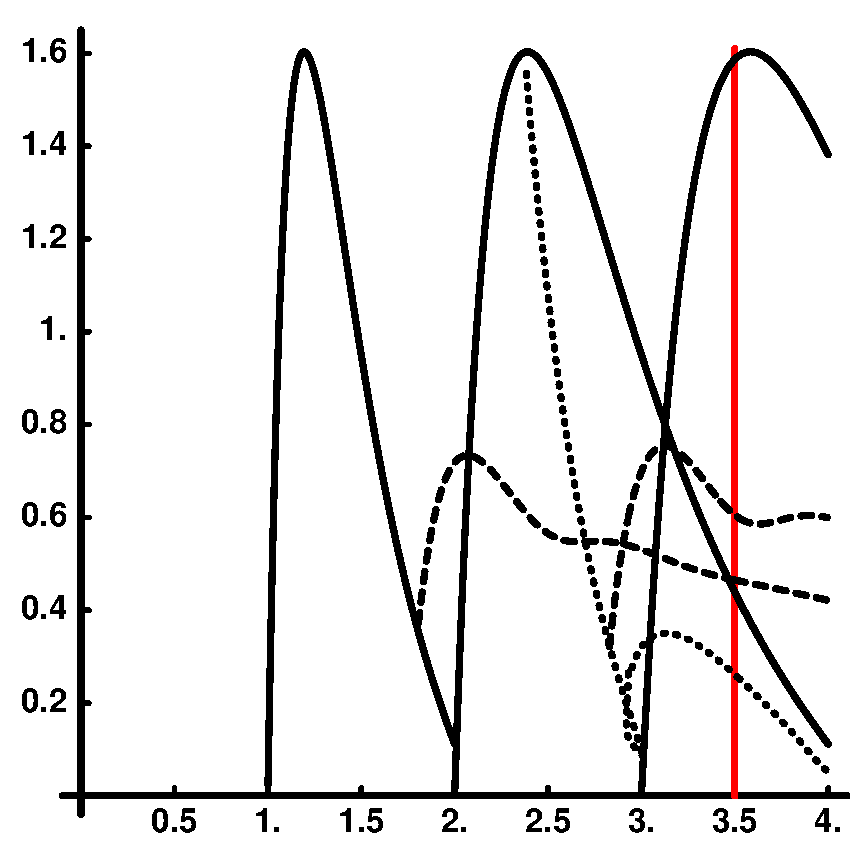
\includegraphics{../../rpo_ks/figs_pst/ksBifDiag}}

\Large

%\psframe*[linecolor=white](-6.5,6)(-5.5,7)
%\psframe*[linecolor=white](6,-6.5)(7.2,-5.5)

\rput(-7.5,0.7){$E$} \rput(0,-7.5){$\tilde{L}$}

\psline[linewidth=1pt]{->}(4.55,-5.7)(5.15,-6.2)\rput(4.25,-5.7){E$_0$}
\psline[linewidth=1pt]{->}(4.55,-4.4)(5.15,-4.1)\rput(4.25,-4.4){E$_1$}
\psline[linewidth=1pt]{->}(4.55,-3.2)(5.15,-2.8)\rput(4.25,-3.25){E$_2$}
\psline[linewidth=1pt]{->}(4.55,6.25)(5.15,6.25)\rput(4.25,6.2){E$_3$}
\psline[linewidth=1pt]{->}(5.85,-2.3)(5.3,-2.5)\rput(6.65,-2.3){TW$_{\pm1}$}
\psline[linewidth=1pt]{->}(5.85,-0.8)(5.3,-1.5)\rput(6.65,-0.8){TW$_{\pm2}$}

\rput(1.75,6.9){C}

% Use grid command below to place objects at specified coordinates.
%\psgrid[subgriddiv=1,griddots=10](-8,-8)(7,7)
}
\end{document}
